\documentclass{article}
\usepackage[letterpaper, margin=1in]{geometry}
\usepackage{fixltx2e}
\usepackage{listings}
\usepackage{graphicx} % Required for inserting images
\usepackage{setspace}
\usepackage{multirow}
\usepackage{float}
\usepackage{biblatex}
\addbibresource{labreport.bib}

\setstretch{1.50}
\title{
\textbf{Laboratory Report} \\
\large Interpolating the elevations into a higher resolution digital elevation matrix M given a lower resolution digital elevation matrix N
}
\author{Jasrel Roby Peralta}
\date{March 2023}

\sloppy
\begin{document}

\maketitle

\section*{Introduction}
\hspace{\parindent} Topographic grid of elevations can be recorded in a form of m $\times$ n matrix. However, lower-resolution matrices cannot provide all elevations of all points in the plot. Through interpolation, more elevation points can be determined to provide a more precise report of datasets. \\
\indent After improving the computer program from the previous exercise, the running time and time complexity of the program are recorded in a table. The data gathered is then used to create charts using graphing software. Different ways of lowering the average running time of the program are also discussed.

\section*{Objectives}
The goal for this exercise is the following:
\begin{itemize}
    \item to determine the average running time and time complexity of the computer program for interpolating the elevation of an \emph{n $\times$ n} square matrix.
    \item to figure out ways to further improve the average running time of the computer program.
\end{itemize}

\section*{Methodology} 
\hspace{\parindent} The machine used for this exercise is running on Ubuntu 22.04.2 LTS x86\_64, Intel i-7 8700 (12 cores) @ 4.60GHz, AMD ATI Radeon HD 8570 / RS 430, with 16GB memory. The programming language used in the computer program is Python 3. The interpolating algorithm used was the Federal Communications Commission (FCC) method. The graphing software used for making the charts is LibreOffice Calc. \\
\indent The program ran three times with the same n value, wherein the recorded times werre averaged. The \emph{n $\times$ n} matrix used in the program started from n valued at 100, up to 1000, incrementing by 100 in each step. Afterward, input sizes doubled in each step until 16000, then lastly interpolated 20000 sized \emph{n $\times$ n} matrix. \\
\indent In getting the theoretical runtimes, the average runtime of the interpolation of the 100 $\times$ 100 matrix served as the base case. The author used \emph{O(n\textsuperscript{2})} as the growth rate of the algorithm. The basis for this decision is the presence of nested loops in the code of the program as seen in the Appendix.

\section*{Results and Discussion}
\hspace{\parindent} After running the program three times, the recorded runtimes of these runs are then averaged. Also, the theoretical runtime for the \emph{n} input size was also determined.
\begin{table}[H]
    \centering
    \begin{tabular}{|c|ccc|c|c|}
    \hline
    \multirow{2}{*}{n} & \multicolumn{3}{c|}{\begin{tabular}[c]{@{}c@{}}runtime\\ (secs)\end{tabular}}     & \multirow{2}{*}{\begin{tabular}[c]{@{}c@{}}average runtime\\ (secs)\end{tabular}} & \multirow{2}{*}{\begin{tabular}[c]{@{}c@{}}theoretical runtime\\ (secs)\end{tabular}} \\ \cline{2-4}
                       & \multicolumn{1}{c|}{r1}          & \multicolumn{1}{c|}{r2}          & r3          &                                                                                   &                                                                                       \\ \hline
    100                & \multicolumn{1}{c|}{0.0162450}   & \multicolumn{1}{c|}{0.0167280}   & 0.0168010   & 0.0165913                                                                         & 0.0165913                                                                             \\ \hline
    200                & \multicolumn{1}{c|}{0.0934830}   & \multicolumn{1}{c|}{0.0608940}   & 0.0604390   & 0.0716053                                                                         & 0.0663653                                                                             \\ \hline
    300                & \multicolumn{1}{c|}{0.1336240}   & \multicolumn{1}{c|}{0.1359470}   & 0.1510750   & 0.1402153                                                                         & 0.1493220                                                                             \\ \hline
    400                & \multicolumn{1}{c|}{0.2496560}   & \multicolumn{1}{c|}{0.2631390}   & 0.2384800   & 0.2504250                                                                         & 0.2654613                                                                             \\ \hline
    500                & \multicolumn{1}{c|}{0.3861530}   & \multicolumn{1}{c|}{0.3845850}   & 0.3695890   & 0.3801090                                                                         & 0.4147833                                                                             \\ \hline
    600                & \multicolumn{1}{c|}{0.5517410}   & \multicolumn{1}{c|}{0.5316630}   & 0.5268450   & 0.5367497                                                                         & 0.5972880                                                                             \\ \hline
    700                & \multicolumn{1}{c|}{0.7228750}   & \multicolumn{1}{c|}{0.7321880}   & 0.7916700   & 0.7489110                                                                         & 0.8129753                                                                             \\ \hline
    800                & \multicolumn{1}{c|}{0.9618760}   & \multicolumn{1}{c|}{0.9641490}   & 1.0071930   & 0.9777393                                                                         & 1.0618453                                                                             \\ \hline
    900                & \multicolumn{1}{c|}{1.1882260}   & \multicolumn{1}{c|}{1.2165920}   & 1.2207670   & 1.2085283                                                                         & 1.3438980                                                                             \\ \hline
    1000               & \multicolumn{1}{c|}{1.5367440}   & \multicolumn{1}{c|}{1.5987220}   & 1.5416220   & 1.5590293                                                                         & 1.6591333                                                                             \\ \hline
    2000               & \multicolumn{1}{c|}{6.3585120}   & \multicolumn{1}{c|}{6.1931260}   & 6.1395040   & 6.2303807                                                                         & 6.6365333                                                                             \\ \hline
    4000               & \multicolumn{1}{c|}{24.8950740}  & \multicolumn{1}{c|}{25.4200880}  & 24.9789970  & 25.0980530                                                                        & 26.5461333                                                                            \\ \hline
    8000               & \multicolumn{1}{c|}{104.6794890} & \multicolumn{1}{c|}{102.5799580} & 103.5682120 & 104.6794890                                                                       & 106.1845333                                                                           \\ \hline
    16000              & \multicolumn{1}{c|}{420.0836360} & \multicolumn{1}{c|}{440.8474390} & 420.1101150 & 427.0137300                                                                       & 424.7381333                                                                           \\ \hline
    20000              & \multicolumn{1}{c|}{647.5259250} & \multicolumn{1}{c|}{678.8252680} & 647.1727770 & 657.8413233                                                                       & 663.6533333                                                                           \\ \hline
    \end{tabular}
    \caption{\label{table}Average and Theoretical runtimes of the program}
\end{table}

\indent To further visualize the results obtained in Table 1, charts for both average runtime and theoretical runtime were created, named Figure 1 and Figure 2, respectively.
\begin{figure}[H]
    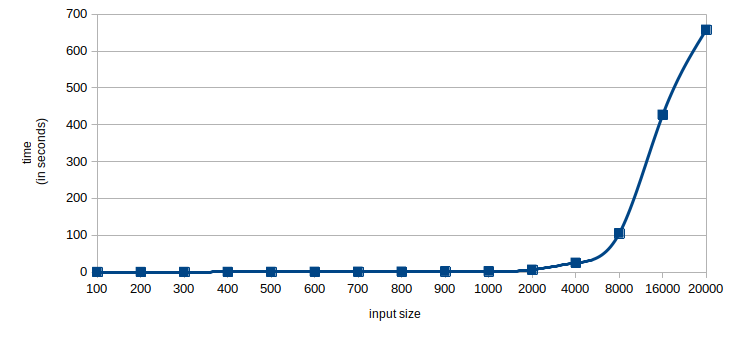
\includegraphics[width=1\textwidth]{chart01.png}
    \centering
    \caption{Line Chart of Average Runtimes}
    \end{figure}

\indent As seen in Figure 1, the chart follows a growth rate similar to the chart presented in Figure 2. Seeing that both line charts agree in form, it can be said that the time complexity of the interpolation of the elevation points of a n $\times$ n square matrix with randomized values at gridpoints divisible by 10 is \emph{O(n\textsuperscript{2})}. \\
\begin{figure}[H]
    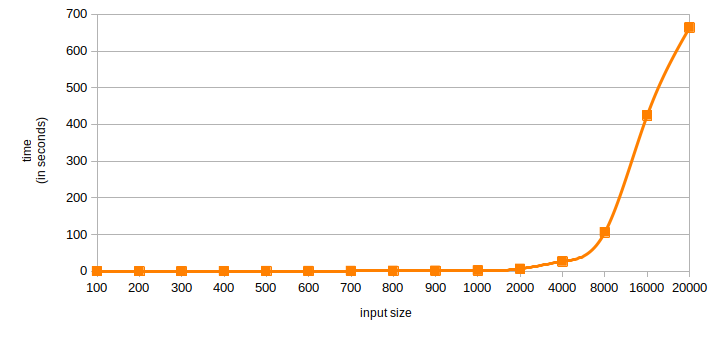
\includegraphics[width=1\textwidth]{chart02.png}
    \centering
    \caption{Line Chart of Theoretical Runtimes}
    \end{figure}


\indent Now that we know the time complexity of the computer program for interpolating elevation points of a n $\times$ n square matrix is \emph{O(n\textsuperscript{2})}, we know that there are ways to further lower the average runtimes of the code. By using better algorithms that employ higher order techniques such as bicubic, and biquintic interpolation, the runtimes of the code are expected to be lesser, even when using larger n inputs~\cite{kidner}. Also, by using a programming language that has a faster compilation time than Python 3, the running time of the code is expected to be much lower~\cite{healthyjournal}.

\section*{Conclusion}
\hspace{\parindent} The runtime of the code of the computer program that interpolates elevation points of a n $\times$ n square matrix is \emph{O(n\textsuperscript{2})}. With this, we know that there are other ways to further improve the runtime of the code. By using other techniques that employ higher orders, and by using another programming language that has a faster compilation time than Python 3, it is expected that the average runtime of the program will be lower.

\printbibliography{}


\pagebreak
\section*{\centering Appendix}
\begin{center}
Interpolation Source Code \\ (main.py)
\end{center}
\setstretch{1}
\begin{lstlisting}[language=Python]
    import numpy as np
    import random
    import datetime
    
    # prettier printing options
    np.set_printoptions(formatter={'float': '{: 0.5f}'.format})
    
    # initialize data
    n = int(input("enter size: "))
    n += 1
    dist = 10
    
    # create a zero nxn matrix
    mat = np.zeros((n,n), dtype = float)
    
    # randomize elevation values for gridpoints divisible by 10
    for i in range(n):
        for j in range(n):
            if i % dist == 0 and j % dist == 0:
                mat[i][j] = random.uniform(0.0, 1000.0)
    
    # for given example in exer file
    # mat[0][0] = 200
    # mat[0][10] = 250
    # mat[10][0] = 280
    # mat[10][10] = 300
    
    # interpolate function
    def terrain_inter(mat):
        for i in range(0,n):
            for j in range(0,n):
                if mat[i][j] != 0:
                    continue
                if (i % dist == 0):
                    get_row_val(i,j)
        for i in range(0,n):
            for j in range(0,n):
                if (mat[i][j] == 0):
                    get_col_val(i,j)
        print("\n")
    
    
    # dp array format:
    # dp = [[x1,y1][x2,y2]]
    
    # interpolate rows with random values
    def get_row_val(i,j):
        dp = get_datapoints_row(i,j)
        x = j               # j -> row
        x1 = dp[0][0]
        x2 = dp[1][0]
        y1 = dp[0][1]
        y2 = dp[1][1]
        res = fcc(x1,y1,x2,y2,x)
        mat[i][j] = res
    
    # interpolate columns
    def get_col_val(i,j):
        dp = get_datapoints_col(i,j)
        # dp = [[x1,y1][x2,y2]]
        x = i               # i -> row
        x1 = dp[0][0]
        x2 = dp[1][0]
        y1 = dp[0][1]
        y2 = dp[1][1]
        res = fcc(x1,y1,x2,y2,x)
        mat[i][j] = res
    
    
    # get closest datapoints to the current gridpoint
    def get_datapoints_row(i,j):
        dp = []
        dp.append(get_nearest_row(i,j,-1))
        dp.append(get_nearest_row(i,j,+1))
        return dp
    def get_datapoints_col(i,j):
        dp = []
        dp.append(get_nearest_col(i,j,-1))
        dp.append(get_nearest_col(i,j,+1))
        return dp
    
    # x, y -> point; dir -> direction 
    # change direction to check to the nearest 10
    ## improved from recursion from previous exercise to direct computation
    def get_nearest_row(i,j,dir):
        # go up
        if dir < 0:
            dir = j - (j % 10)
        # go down
        else:
            dir = j + (10 - (j % 10))
        return [dir,mat[i][dir]]
    
    def get_nearest_col(i,j,dir):
        # go left
        if dir < 0:
            dir = i - (i % 10)
        # go right
        else:
            dir = i + (10 - (i % 10))
        return [dir,mat[dir][j]]
    
    # follow given FCC formula
    def fcc(x1,y1,x2,y2,x):
        return (y1 + (((x-x1)/(x2-x1)) * (y2-y1)))
    
    # print initial matrix
    print(mat)
    
    # record time before interpolation
    time_before = datetime.datetime.now()
    
    # interpolate matrix
    terrain_inter(mat)
    
    # record time after interpolation
    time_after = datetime.datetime.now()
    
    # print interpolation time
    print(time_after-time_before)
    
    # print resulting matrix
    print(mat)
\end{lstlisting}

\end{document}
